% small.tex
\documentclass{beamer}
%\usetheme{default}
\usetheme{Warsaw}
\usecolortheme{whale}
\usepackage{tikz}
\usepackage[absolute,overlay]{textpos}
\usepackage{soul}
\usepackage{pdfpages}
\usepackage[most]{tcolorbox}
%\usepackage{multirow}
\usepackage{tikz,amsmath,array}


\newcommand{\greekbf}[1]{\boldsymbol{\mathrm{#1}}}
\newcommand{\btVFill}{\vskip0pt plus 1filll}
\newcolumntype{P}[1]{>{\centering\arraybackslash}p{#1}}

%\setbeamertemplate{background}[grid][step=.25\textwidth]

\title[selection]{Action of selection on fertility and mortality}
%\subtitle
\author{Michael Holton Price}
\institute[SFI] {
	Santa Fe Institute\\
	MichaelHoltonPrice@gmail.com\\
	\line(1,0){0}\\
	SFI Population Short Course\\
	16 Oct 2018\\
}
%\date{05 Feb 2014}
\date{}

% Note: default dimensions are 128 mm by 96 mm (4 x 3)
\begin{document}

%----------- titlepage ----------------------------------------------%
\begin{frame}[plain]
  \titlepage
\end{frame}

%----------- slide --------------------------------------------------%
\begin{frame}
  \frametitle{Guessing game}
  % 5 kg / 17.3 yr
  % 36 kg / 20.8 yr
  % 800 kg / 39.5 yr
  \begin{columns}[c]
   \column{.33\textwidth}
     \begin{block}{Dik dik}
      \begin{center}
        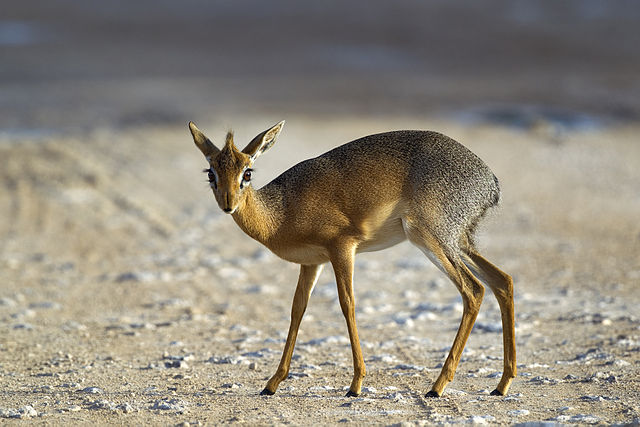
\includegraphics[height=.25\textheight]{640px-Madoqua_kirkii_-_female_(Namutoni).jpg}\
      \end{center}
      5 kg
    \end{block}
    
     \column{.33\textwidth}
     \begin{block}{Chital}
      \begin{center}
        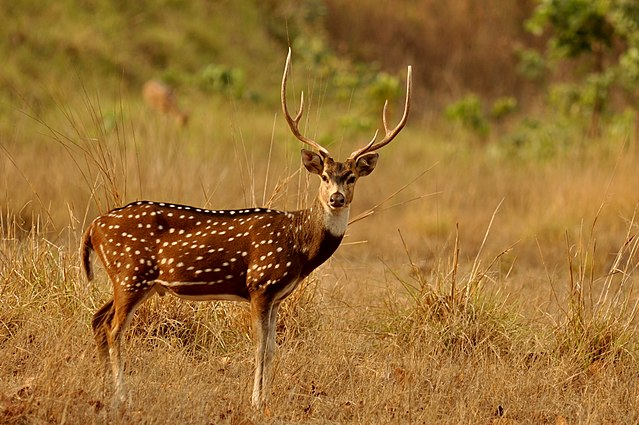
\includegraphics[height=.25\textheight]{640px-A_chital_stag_1.jpg}\
      \end{center}
      36 kg
    \end{block}

   \column{.33\textwidth}
     \begin{block}{Giraffe}
      \begin{center}
        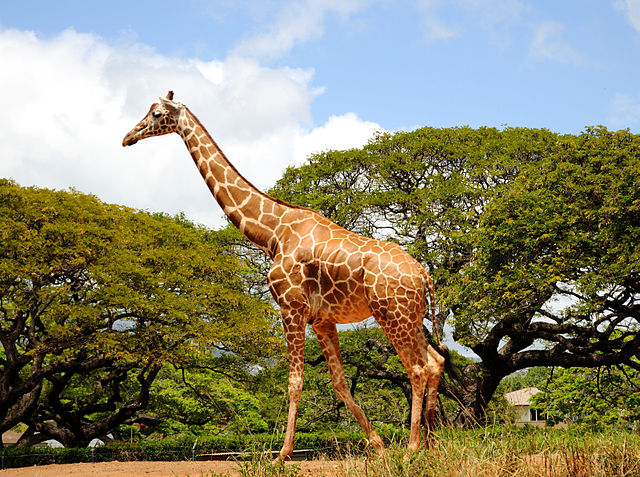
\includegraphics[height=.25\textheight]{640px-Giraffe!_(4565230826).jpg}\
      \end{center}
      800 kg
    \end{block}
  \end{columns}

  \btVFill
  \small Images from Wikipedia \normalsize
\end{frame}

%----------- slide --------------------------------------------------%
\begin{frame}
  \frametitle{Guessing game}
  % 5 kg / 17.3 yr
  % 36 kg / 20.8 yr
  % 800 kg / 39.5 yr
  \begin{columns}[c]
   \column{.33\textwidth}
     \begin{block}{Dik dik}
      \begin{center}
        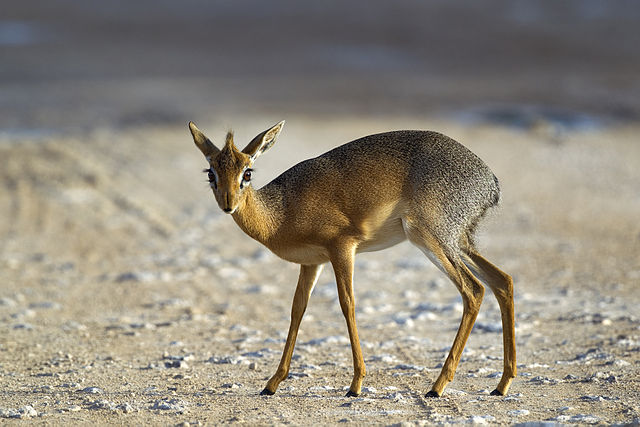
\includegraphics[height=.25\textheight]{640px-Madoqua_kirkii_-_female_(Namutoni).jpg}\
      \end{center}
      5 kg
    \end{block}
    
     \column{.33\textwidth}
     \begin{block}{Chital}
      \begin{center}
        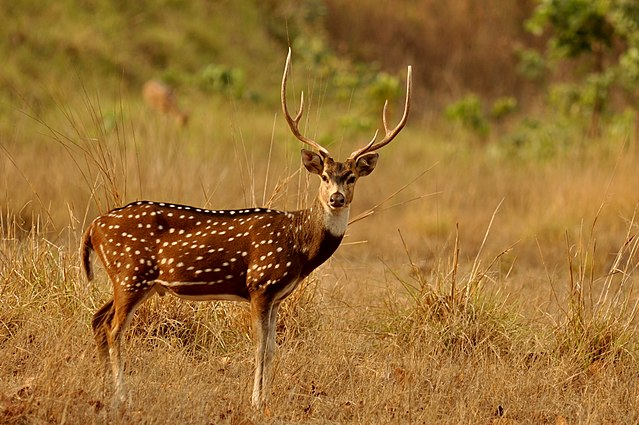
\includegraphics[height=.25\textheight]{640px-A_chital_stag_1.jpg}\
      \end{center}
      36 kg  \hfill 20.8 yr
    \end{block}

   \column{.33\textwidth}
     \begin{block}{Giraffe}
      \begin{center}
        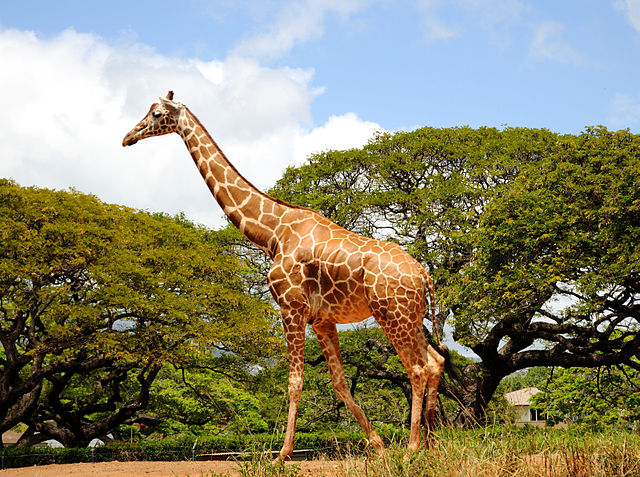
\includegraphics[height=.25\textheight]{640px-Giraffe!_(4565230826).jpg}\
      \end{center}
      800 kg
    \end{block}
  \end{columns}

  \btVFill
  \small Images from Wikipedia \normalsize
\end{frame}

%----------- slide --------------------------------------------------%
\begin{frame}
  \frametitle{Guessing game}
  % 5 kg / 17.3 yr
  % 36 kg / 20.8 yr
  % 800 kg / 39.5 yr
  \begin{columns}[c]
   \column{.33\textwidth}
     \begin{block}{Dik dik}
      \begin{center}
        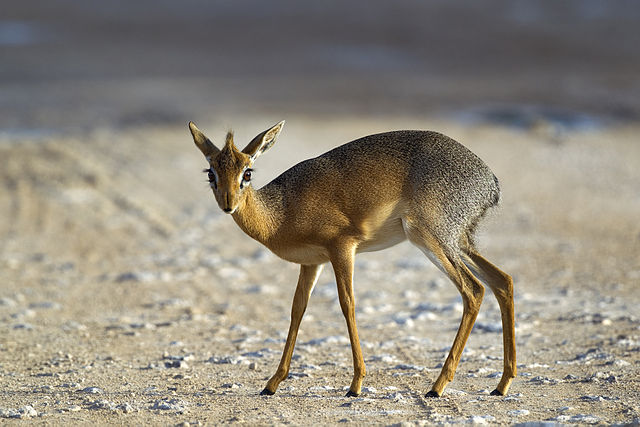
\includegraphics[height=.25\textheight]{640px-Madoqua_kirkii_-_female_(Namutoni).jpg}\
      \end{center}
      5 kg
    \end{block}
    
     \column{.33\textwidth}
     \begin{block}{Chital}
      \begin{center}
        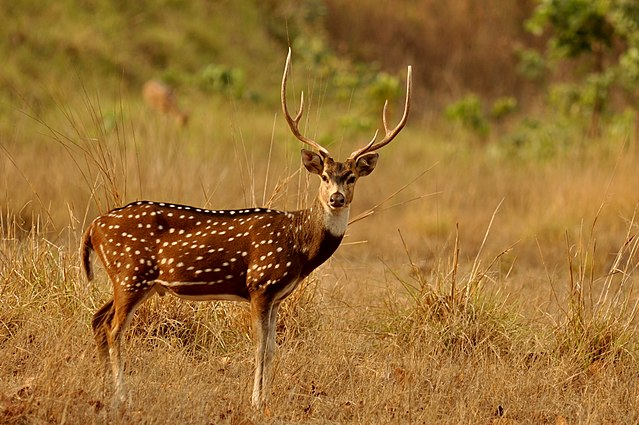
\includegraphics[height=.25\textheight]{640px-A_chital_stag_1.jpg}\
      \end{center}
      36 kg  \hfill 20.8 yr
    \end{block}

   \column{.33\textwidth}
     \begin{block}{Giraffe}
      \begin{center}
        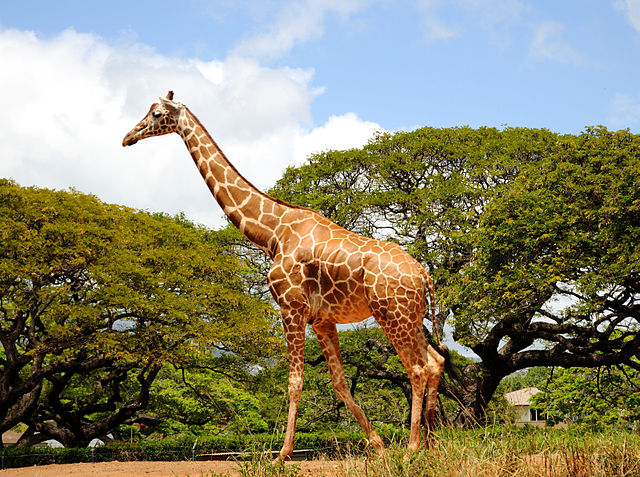
\includegraphics[height=.25\textheight]{640px-Giraffe!_(4565230826).jpg}\
      \end{center}
      800 kg \hfill 39.5 yr
    \end{block}
  \end{columns}

  \btVFill
  \small Images from Wikipedia \normalsize
\end{frame}

%----------- slide --------------------------------------------------%
\begin{frame}
  \frametitle{Guessing game}
  % 5 kg / 17.3 yr
  % 36 kg / 20.8 yr
  % 800 kg / 39.5 yr
  \begin{columns}[c]
   \column{.33\textwidth}
     \begin{block}{Dik dik}
      \begin{center}
        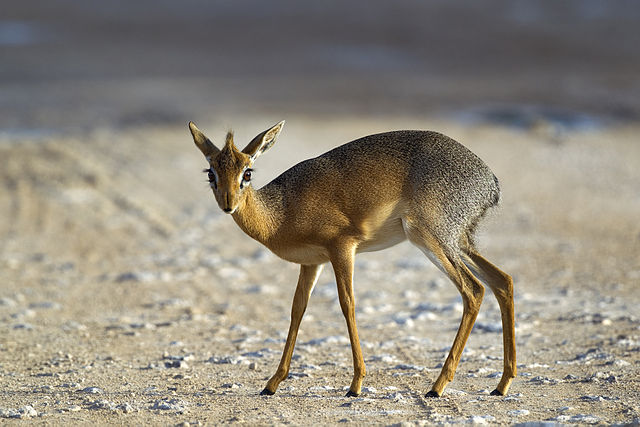
\includegraphics[height=.25\textheight]{640px-Madoqua_kirkii_-_female_(Namutoni).jpg}\
      \end{center}
      5 kg \hfill 17.3 yr
    \end{block}
    
     \column{.33\textwidth}
     \begin{block}{Chital}
      \begin{center}
        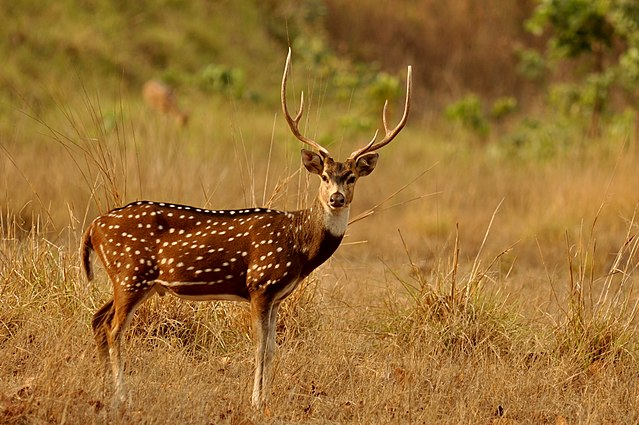
\includegraphics[height=.25\textheight]{640px-A_chital_stag_1.jpg}\
      \end{center}
      36 kg  \hfill 20.8 yr
    \end{block}

   \column{.33\textwidth}
     \begin{block}{Giraffe}
      \begin{center}
        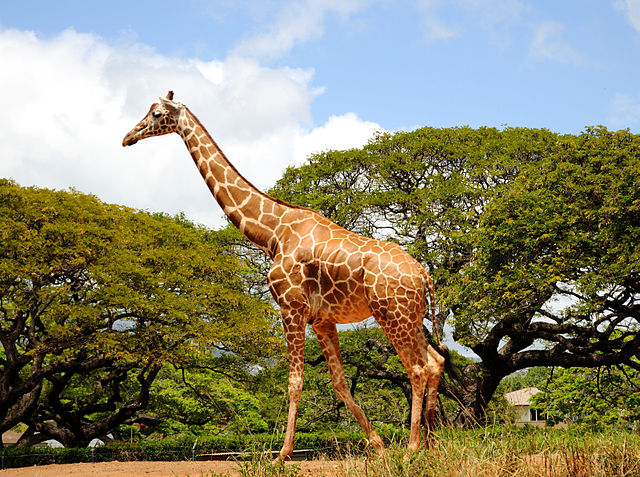
\includegraphics[height=.25\textheight]{640px-Giraffe!_(4565230826).jpg}\
      \end{center}
      800 kg \hfill 39.5 yr
    \end{block}
  \end{columns}

  \btVFill
  \small Images from Wikipedia \normalsize
\end{frame}
%----------- slide --------------------------------------------------%
\begin{frame}{Life history theory}
How natural selection shapes life histories
\end{frame}

%----------- slide --------------------------------------------------%
\begin{frame}{Life history traits}
Growth pattern\\
\pause
\vspace{1cm}
Lifespan\\
\pause
\vspace{1cm}
Age at maturity\\
\pause
\vspace{1cm}
Size at independence and maturity\\
\pause
\vspace{1cm}
Age- and size-specific reproductive effort and mortality schedules\\
\end{frame}

%----------- slide --------------------------------------------------%
\begin{frame}{Trade-offs: Constrained optimization}
Graph here\\
\end{frame}

\begin{frame}{Energy / effort partition models}
Graph here\\
\end{frame}

\begin{frame}{Energy / effort partition models}
Example?\\
\end{frame}

\begin{frame}{The space of mammalian life history traits}
Four graphs\\
\end{frame}

\begin{frame}{People are weird}
Four graphs\\
\end{frame}

\begin{frame}{Linking economic and evolutionary theory: evolution of time preference}
Core results and graphs\\
\end{frame}

%----------- slide --------------------------------------------------%
\begin{frame}{Reproductive Value: ``important but confusing concept''}
\begin{block}{Euler 1930}
``We may ask, not only about the newly born, but about persons of any chosen age, what is the present value of their future offspring; and if the present value is calculated at the rate determined as before, the question has the definite meaning -- To what extent will persons of this age, on the average, contribute to the ancestry of future generations? The question is one of some interest, since the direct action of Natural Selection must be proportional to this contribution.''
\end{block}
\vspace{.5cm}
\pause
% "easily seen to be given by this equation"
$\frac{v(x)}{v(0)} = \frac{e^{rx}}{l(x)} \int_{x}^{\infty} e^{-ra} \, l(a) \, m(a) \, da$
\end{frame}

%----------- slide --------------------------------------------------%
\begin{frame}{Reproductive Value: discrete age classes}
  $v_i =  \displaystyle\sum\limits_{j=i}^{J} \frac{P_{ij} \, F_j}{\lambda^{j-i+1}} = \frac{F_i}{\lambda} + \frac{P_{i+1} \, F_{i+1}}{\lambda^2} + \frac{P_{i+1} \, P_{i+2} \, F_{i+2}}{\lambda^3} + \cdots$\\
  \vspace{.5cm}
  where\\
  \vspace{.5cm}
  $P_j$ is age-specific survival\\
  \vspace{.5cm}
  $F_j$ is age-specific fertility\\
  \vspace{.5cm}
  $P_{ij} = P_i \, P_{i+1} \cdots P_{j-1}$ is survival from age class $i$ to $j$\\
  \vspace{.5cm}
  $\lambda$ is the per period growth rate\\
\end{frame}

%----------- slide --------------------------------------------------%
\begin{frame}{Repro value plots using Goodman data}
\end{frame}

%----------- slide --------------------------------------------------%
\begin{frame}{Euler-Lotka / characteristic equation}
  $v_1 = 1 = \displaystyle\sum\limits_{j=1}^{J} \frac{P_{1j} \, F_j}{\lambda^j} = \displaystyle\sum\limits_{j=1}^{J} \frac{l_j \, F_j}{\lambda^j}$\\
\vspace{.5cm}
where\\
\vspace{.5cm}
  $l_j = P_{1j}$ is survival from birth to age class $j$\\
\end{frame}

%----------- slide --------------------------------------------------%
\begin{frame}{Euler-Lotka continuous form}
  $1 = \int_{0}^{\infty} e^{-ra} \, l(a) \, b(a) da$\\
\end{frame}

%----------- slide --------------------------------------------------%
\begin{frame}{Euler-Lotka meets scaling theory}
\end{frame}

%----------- slide --------------------------------------------------%
{
  \setbeamercolor{background canvas}{bg=}
  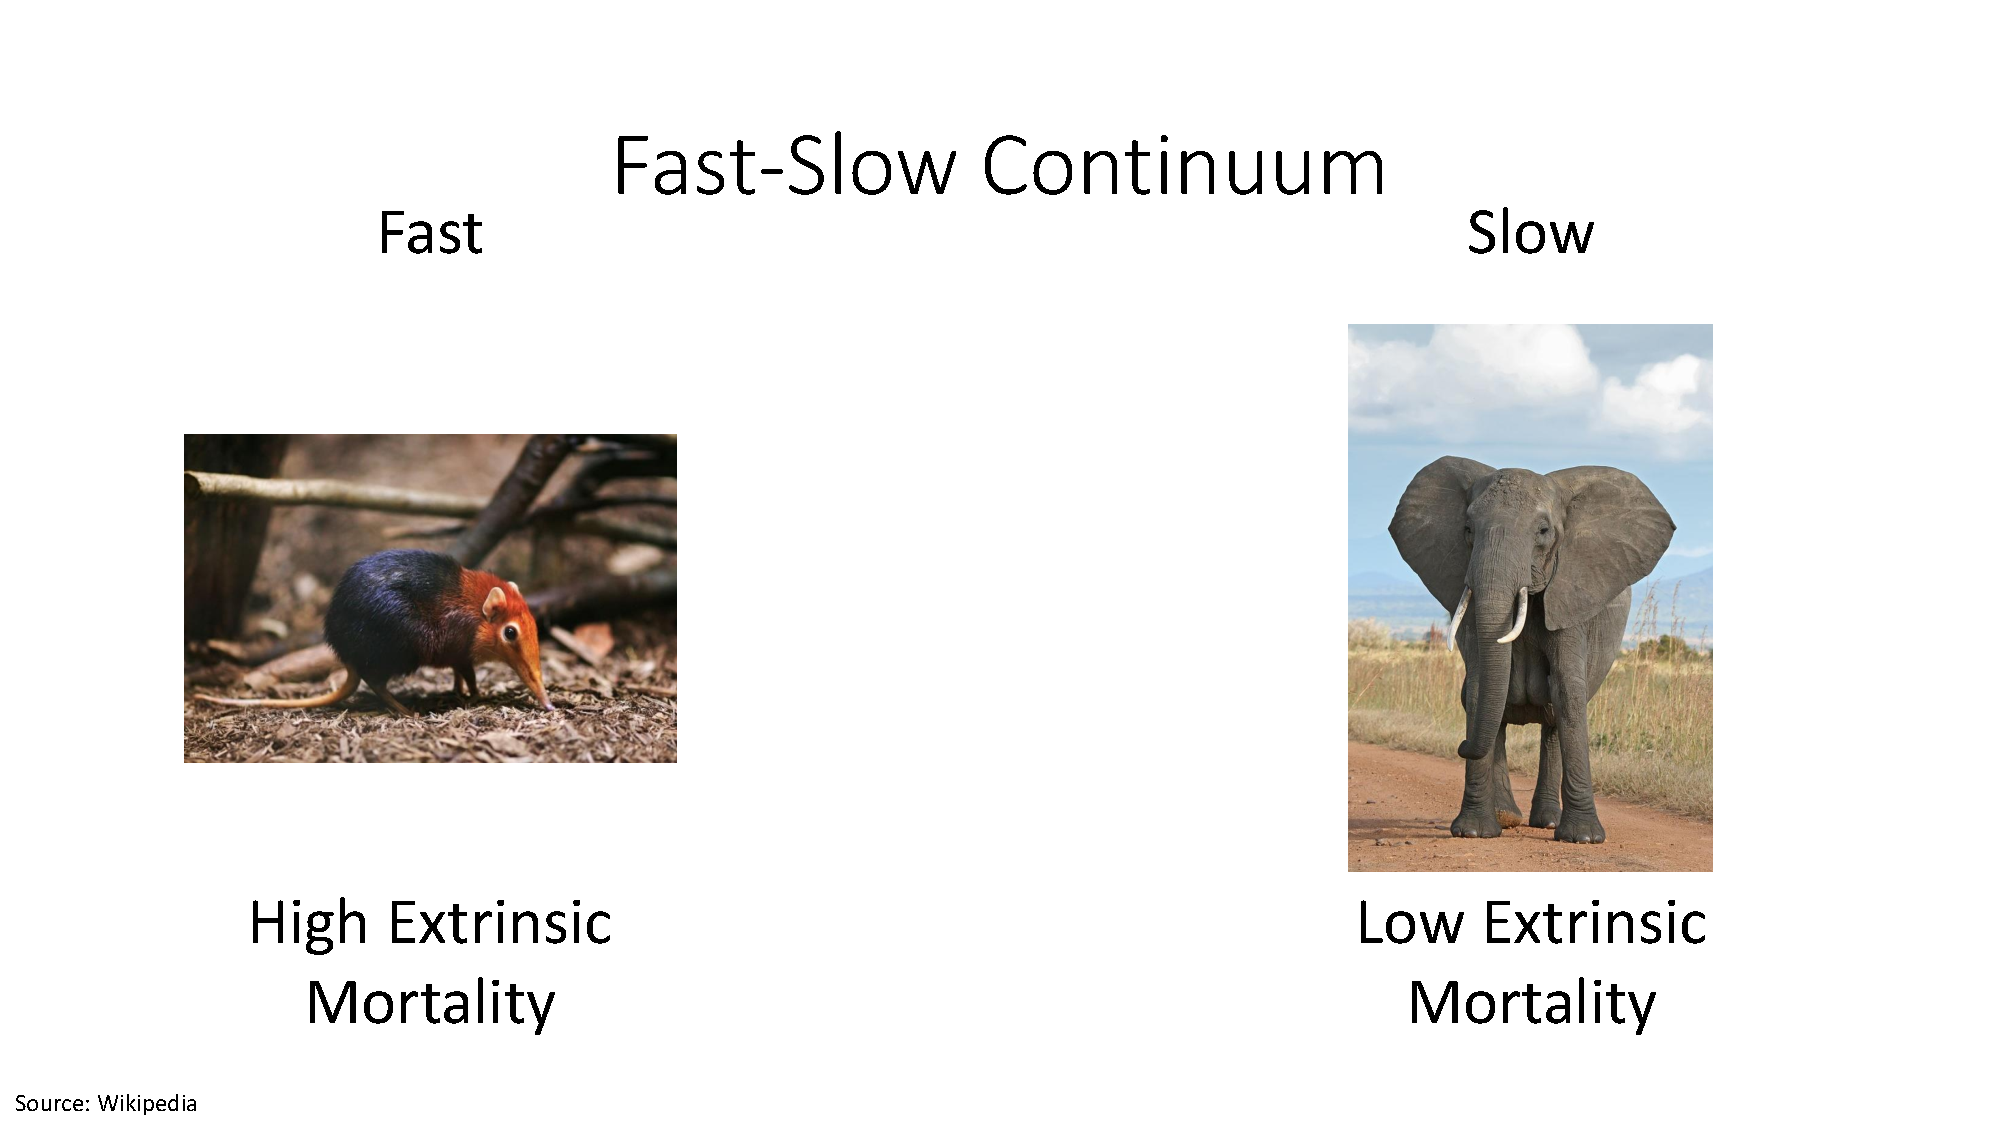
\includepdf[pages=1-9]{princeton_select_slides.pdf}
}

%----------- slide --------------------------------------------------%
\begin{frame}{Euler-Lotka meets scaling theory}
  $1 = e^{-r \alpha} \, R(w_0,w_{\alpha}) \, V(w_0,w_{\alpha})$\\
  \vspace{.5cm}
  \pause
  $r = r(w_0,w_{\alpha})$\\
  \vspace{.5cm}
  \pause
  $\frac{\partial r}{\partial w_0} = 0$\\
  \vspace{.5cm}
  \pause
  $\alpha = \alpha(w_0,w_{\alpha})$\\
  \vspace{.5cm}
  \pause
  $\frac{\partial}{\partial w_0} \left[ e^{-r \alpha} \, R(w_0,w_{\alpha}) \, V(w_0,w_{\alpha}) \right] = 0$\\
  \vspace{.5cm}
  \pause
  $\frac{\partial \log{R}}{\partial w_0} - r \, \frac{\partial \alpha}{\partial w_0} + \frac{\partial \log{V}}{\partial w_0} \log{R} = 0$\\
\end{frame}

%----------- slide --------------------------------------------------%
{
  \setbeamercolor{background canvas}{bg=}
  \includepdf[pages=10]{princeton_select_slides.pdf}
}

%%----------- slide --------------------------------------------------%
%\begin{frame}{$R_0$: Expected daughters across mother's lifespan}
%$1 = \displaystyle\sum\limits_{j=1}^{J} \frac{l_j \, b_j}{\lambda^j}$\\
%\vspace{.5cm}
%Compare to:\\
%\vspace{.5cm}
%$R_0 = \displaystyle\sum\limits_{j=1}^{J} l_j \, b_j$\\
%\end{frame}

%----------- slide --------------------------------------------------%
\begin{frame}{Leslie matrix formalism inherently satisfies Euler-Lotka equation}
Given stable demography\\
\end{frame}

%----------- slide --------------------------------------------------%
\begin{frame}{Review: Leslie Matrices}
\centering
\begin{equation*}
	\label{eq:A}
	\mathbf{A} = 
	\left( \begin{array}{cccccc}
		F_1 & F_2 & F_3 & F_4    & \cdots  & F_{J}   \\
		P_1 & 0   & 0   & 0      & \cdots  & 0       \\
		0   & P_2 & 0   & 0      & \cdots  & 0       \\
		0   & 0   & P_3 & 0      & \cdots  & 0       \\
		0   & 0   & 0   & \ddots & \cdots  & 0       \\
		0   & 0   & 0   & \ddots & P_{J-1} & 0
	\end{array} \right)
\end{equation*}
\\
\pause
\vspace{1.5cm}
$\mathbf{z}_{t+1} = \mathbf{A} \, \mathbf{z}_t$
\end{frame}

\begin{frame}{Leslie to Euler-Lotka}
  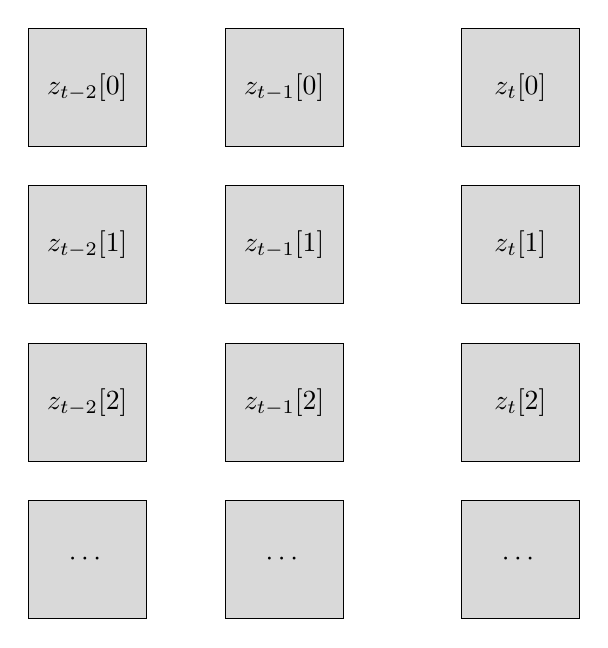
\begin{tikzpicture}[every text node part/.style={align=center}]
    % Preliminaries
    \usetikzlibrary{shapes.geometric, arrows, shapes.multipart}
    \tikzstyle{box} = [rectangle, minimum width=1.5cm, minimum height=1.5cm, text centered, draw=black, fill=gray!30]
    %\tikzstyle{box} = [rectangle, minimum width=1.5cm, minimum height=1cm, text centered, draw=black, fill=orange!30]
    \tikzstyle{strat} = [rectangle, minimum width=1.5cm, minimum height=1cm, text centered, draw=white, fill=white]
    \tikzstyle{arrow} = [thick,->,>=stealth]
    % Field Processing Flow
    %\node (field_strat) [strat] {Field \\ Processing};
    \node (z_tm2_0) [box] {$z_{t-2}[0]$};
    \pause
    \node (z_tm2_1) [box,below of=z_tm2_0,yshift=-1cm] {$z_{t-2}[1]$};
    \pause
    \node (z_tm2_2) [box,below of=z_tm2_1,yshift=-1cm] {$z_{t-2}[2]$};
    \pause
    \node (z_tm2_3) [box,below of=z_tm2_2,yshift=-1cm] {$\cdots$};
    \pause
    \node (z_tm1_0) [box,right of=z_tm2_0,xshift=1.5cm] {$z_{t-1}[0]$};
    \node (z_tm1_1) [box,below of=z_tm1_0,yshift=-1cm] {$z_{t-1}[1]$};
    \node (z_tm1_2) [box,below of=z_tm1_1,yshift=-1cm] {$z_{t-1}[2]$};
    \node (z_tm1_3) [box,below of=z_tm1_2,yshift=-1cm] {$\cdots$};
    \pause
    \node (z_t_0) [box,right of=z_tm1_0,xshift=2cm] {$z_t[0]$};
    \node (z_t_1) [box,below of=z_t_0,yshift=-1cm] {$z_t[1]$};
    \node (z_t_2) [box,below of=z_t_1,yshift=-1cm] {$z_t[2]$};
    \node (z_t_3) [box,below of=z_t_2,yshift=-1cm] {$\cdots$};
    \pause
  \end{tikzpicture}
\end{frame}

\begin{frame}{Leslie to Euler-Lotka}
  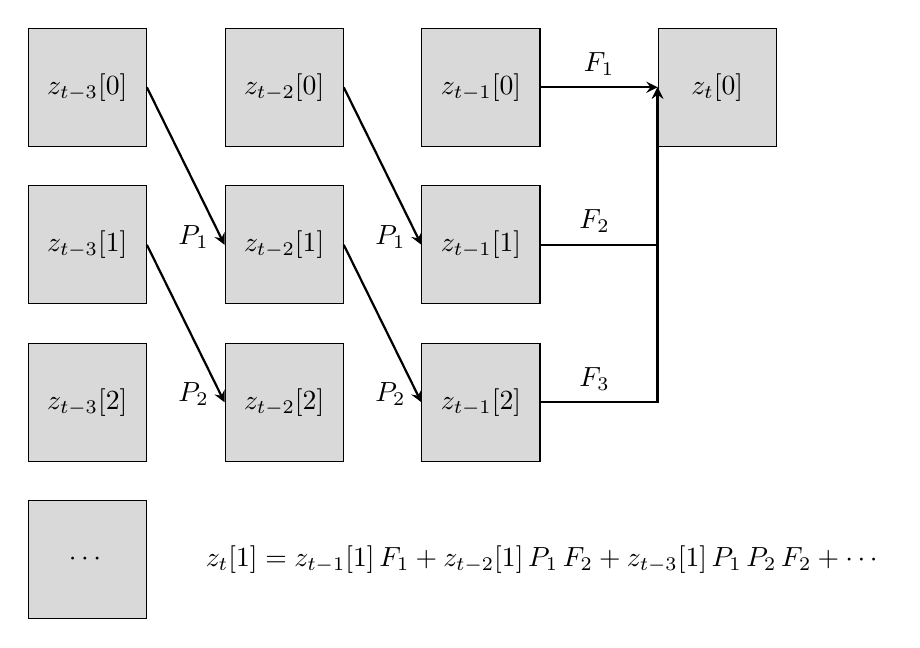
\begin{tikzpicture}[every text node part/.style={align=center}]
    % Preliminaries
    \usetikzlibrary{shapes.geometric, arrows, shapes.multipart}
    \tikzstyle{box} = [rectangle, minimum width=1.5cm, minimum height=1.5cm, text centered, draw=black, fill=gray!30]
    %\tikzstyle{box} = [rectangle, minimum width=1.5cm, minimum height=1cm, text centered, draw=black, fill=orange!30]
    \tikzstyle{mathbox} = [rectangle, minimum width=1.5cm, minimum height=1cm, text centered, draw=white, fill=white]
    \tikzstyle{arrow} = [thick,->,>=stealth]
    % Field Processing Flow
    %\node (field_strat) [strat] {Field \\ Processing};
    \node (z_tm3_0) [box] {$z_{t-3}[0]$};
    \node (z_tm3_1) [box,below of=z_tm3_0,yshift=-1cm] {$z_{t-3}[1]$};
    \node (z_tm3_2) [box,below of=z_tm3_1,yshift=-1cm] {$z_{t-3}[2]$};
    \node (z_tm3_3) [box,below of=z_tm3_2,yshift=-1cm] {$\cdots$};
    
    \node (z_tm2_0) [box,right of=z_tm3_0,xshift=1.5cm] {$z_{t-2}[0]$};
    \node (z_tm2_1) [box,below of=z_tm2_0,yshift=-1cm] {$z_{t-2}[1]$};
    \node (z_tm2_2) [box,below of=z_tm2_1,yshift=-1cm] {$z_{t-2}[2]$};
    %\node (z_tm2_4) [box,below of=z_tm2_3,yshift=-1cm] {$\cdots$};
    
    \node (z_tm1_0) [box,right of=z_tm2_0,xshift=1.5cm] {$z_{t-1}[0]$};
    \node (z_tm1_1) [box,below of=z_tm1_0,yshift=-1cm] {$z_{t-1}[1]$};
    \node (z_tm1_2) [box,below of=z_tm1_1,yshift=-1cm] {$z_{t-1}[2]$};
    %\node (z_tm1_4) [box,below of=z_tm1_3,yshift=-1cm] {$\cdots$};
    
    \node (z_t_0) [box,right of=z_tm1_0,xshift=2cm] {$z_t[0]$};
    
    \draw [arrow] (z_tm3_0.east) to node[xshift=.1cm,yshift=-.9cm] {$P_1$} (z_tm2_1.west);
    \pause
    \draw [arrow] (z_tm3_1.east) to node[xshift=.1cm,yshift=-.9cm] {$P_2$} (z_tm2_2.west);
    %\draw [arrow] (z_tm2_3.east) to (z_tm1_4.west);
    \pause

    \draw [arrow] (z_tm2_0.east) to node[xshift=.1cm,yshift=-.9cm] {$P_1$} (z_tm1_1.west);
    \draw [arrow] (z_tm2_1.east) to node[xshift=.1cm,yshift=-.9cm] {$P_2$} (z_tm1_2.west);
    %\draw [arrow] (z_tm1_3.east) to (z_t_4.west);
    \pause
    
    \draw [arrow] (z_tm1_0.east) to node[yshift=.3cm] {$F_1$} (z_t_0.west);
    \draw [arrow] (z_tm1_1.east) -| node[yshift=.3cm,xshift=-.8cm] {$F_2$} (z_t_0.west);
    \draw [arrow] (z_tm1_2.east) -| node[yshift=.3cm,xshift=-.8cm] {$F_3$} (z_t_0.west);
    
    \node (euler_lotka) [mathbox,right of=z_tm3_3,xshift=4.8cm] {$z_t[1] = z_{t-1}[1] \, F_1 + z_{t-2}[1] \, P_1 \, F_2 + z_{t-3}[1] \, P_1 \, P_2 \, F_2 + \cdots$};
    
  \end{tikzpicture}
\end{frame}

\begin{frame}{Leslie to Euler-Lotka}
  $y_t \equiv z_t[1]$\\
  \vspace{.5cm}
  $y_t = y_{t-1} \, F_1 + y_{t-2} \, S_1 \ F_2 + y_{t-2} \, P_1 \, P_2 \, F_3 + \cdots = \displaystyle\sum\limits_{j=1}^{J} y_{t-j-1} \, l_j \, F_j$\\
  \vspace{.5cm}
  Posit an exponential solution\\
  \vspace{.5cm}
  $y_{t-j-1} = \frac{y_t}{\lambda^{j+1}}$\\
  \vspace{.5cm}
  $1 = \displaystyle\sum\limits_{j=1}^{J} \frac{l_j \, F_j}{\lambda^{j+1}}$\\
  %$l_j = \displaystyle\prod\limits_{i=1}^{j-1} P_k$
\end{frame}

\begin{frame}{Starting with Leslie usually simplifies life}
  Though, this requires familiarity with linear algebra and multivariable calculus
\end{frame}

\begin{frame}{Aside: derivatives of matrices}
  The right eigenvectors of $\mathbf{A}$ are defined by the equation\\
  \vspace{.5cm}
  $\mathbf{A} \, \mathbf{w}^{(m)} = \lambda^{(m)} \, \mathbf{w}^{(m)}$\\
  \vspace{.5cm}
  The left eigenvectors of $\mathbf{A}$ are defined by the equation\\
  ${\mathbf{v}^{(m)}}^{\dagger} \, \mathbf{A} =	{\mathbf{v}^{(m)}}^{\dagger} \, \lambda^{(m)}$\\
  \vspace{.5cm}
  Taking an exterior derivative of the top equation yields\\
  \vspace{.5cm}
  $\mathrm{d}\mathbf{A} \, \mathbf{w}^{(m)} + \mathbf{A} \, \mathrm{d}\mathbf{w}^{(m)}= \mathrm{d}\lambda^{(m)} \, \mathbf{w}^{(m)} + \lambda^{(m)} \, \mathrm{d}\mathbf{w}^{(m)}$\\
\end{frame}

\begin{frame}{Aside: derivatives of matrices}
  Now take the inner product with respect to $\greekbf{v}^{(n)}$ (i.e., pre-multiply by ${\greekbf{v}^{(n)}}^{\dagger}$ and rearrange terms)\\
  \vspace{.5cm}
  ${\mathbf{v}^{(n)}}^{\dagger} \, \mathrm{d}\mathbf{A} \, \mathbf{w}^{(m)} = {\mathbf{v}^{(n)}}^{\dagger} \, \mathrm{d}\lambda^{(m)} \, \mathbf{w}^{(m)} + {\mathbf{v}^{(n)}}^{\dagger} \left(\lambda^{(m)} - \mathbf{A} \right) \mathrm{d}\mathbf{w}^{(m)}$\\
  \vspace{.5cm}
  If $m=n$ the last term on the right vanishes\\
  \vspace{.5cm}
  ${\mathbf{v}^{(m)}}^{\dagger} \, \mathrm{d}\mathbf{A} \, \mathbf{w}^{(m)} = {\mathbf{v}^{(m)}}^{\dagger} \, \mathrm{d}\lambda^{(m)} \, \mathbf{w}^{(m)}$\\
\end{frame}

\begin{frame}{Aside: derivatives of matrices}
  Solving for $\mathrm{d}\lambda^{(m)}$ yields\\
  \vspace{.5cm}
  $\mathrm{d}\lambda^{(m)} = \frac{{\mathbf{v}^{(m)}}^{\dagger} \, \mathrm{d}\mathbf{A} \, \mathbf{w}^{(m)}}{\psi^{(m)}}$\\
  \vspace{.5cm}
  where $\psi^{(m)}=\mathbf{v}^{(m)\dagger} \, \mathbf{w}^{(m)}$ is the inner product of the left and right eigenvectors of $\lambda^{(m)}$.\\
  \vspace{.5cm}
  Representing this in terms of the matrix element $A_{ij}$ yields\\
  \vspace{.5cm}
  $\frac{\partial \lambda^{(m)}}{\partial A_{ij}} = \frac{v^{(m)}_i \, w^{(m)}_j}{\psi^{(m)}}$
\end{frame}

\begin{frame}{Amazingly}
  $\mathbf{v}$, the domimant left eigenvector of $\mathbf{A}$, is the vector of age-specific reproductive values\\
  \vspace{.5cm}
  Less amazingly (perhaps):\\
  \vspace{.5cm}
  $\mathbf{w}$, the domimant right eigenvector of $\mathbf{A}$, is the stable age distribution\\
  \vspace{.5cm}
  Remarkably (perhaps) the derivative of the dominant eigenvalue with respect to any matrix element is\\
  \vspace{.5cm}
  $\frac{\partial \lambda}{\partial A_{ij}} = \frac{v_i \, w_j}{\psi}$
\end{frame}

\begin{frame}{Use this to link evolutionary and economic theory}
Assume that each element of the Leslie matrix depends on a valuable but limited resource that can be used to increase its value. Stated formally, each Leslie matrix element $A_{i'i}$ is a monotonically increasing function of consumption allocated to it, $x_{i'i}$. For example, an individual can increase survival in a given age class by dedicating more resources to it and, similarly, can increase fertility by dedicating more resources to reproduction. These scarce resources can be re-allocated between any two matrix elements, both inter-temporally and between survival and fertility in the same age class. Given these preliminaries, it is straightforward to derive the intertemporal MRS at constant fitness ($d\lambda=0$) using the chain rule. 
\end{frame}

\begin{frame}{Use this to link evolutionary and economic theory}
  $MRS_{\lambda} = -\frac{dx_{j'j}}{dx_{i'i}}\bigg|_{d\lambda=0} = \frac{\frac{\partial \lambda}{\partial A_{i'i}}}{\frac{\partial \lambda}{\partial A_{j'j}}} \frac{\frac{\partial A_{i'i}}{\partial x_{i'i}}}{\frac{\partial A_{j'j}}{\partial x_{j'j}}} = \frac{v_{i'} \, w_i}{v_{j'} \, w_j} \frac{A'_{i'i}}{A'_{j'j}}$\\
  \vspace{.5cm}
  Representing this in terms of only fertility or only survival yields\\
  \vspace{.5cm}
  $MRS_{\lambda,ij} = \frac{w_i}{w_j} \frac{F'_i}{F'_j} = \frac{v_{i+1}}{v_{j+1}} \frac{w_i}{w_j} \frac{P'_i}{P'_j}$\\
  \vspace{.5cm}
  Emplying some identities:\\
  \vspace{.5cm}
  $MRS_{\lambda,ij} = \frac{1}{P_{ij}} \lambda^{j-i} \frac{F'_i}{F'_j}$
\end{frame}



\end{document}
